% Options for packages loaded elsewhere
\PassOptionsToPackage{unicode}{hyperref}
\PassOptionsToPackage{hyphens}{url}
\PassOptionsToPackage{dvipsnames,svgnames*,x11names*}{xcolor}
%
\documentclass[
]{article}
\usepackage{lmodern}
\usepackage{amssymb,amsmath}
\usepackage{ifxetex,ifluatex}
\ifnum 0\ifxetex 1\fi\ifluatex 1\fi=0 % if pdftex
  \usepackage[T1]{fontenc}
  \usepackage[utf8]{inputenc}
  \usepackage{textcomp} % provide euro and other symbols
\else % if luatex or xetex
  \usepackage{unicode-math}
  \defaultfontfeatures{Scale=MatchLowercase}
  \defaultfontfeatures[\rmfamily]{Ligatures=TeX,Scale=1}
\fi
% Use upquote if available, for straight quotes in verbatim environments
\IfFileExists{upquote.sty}{\usepackage{upquote}}{}
\IfFileExists{microtype.sty}{% use microtype if available
  \usepackage[]{microtype}
  \UseMicrotypeSet[protrusion]{basicmath} % disable protrusion for tt fonts
}{}
\makeatletter
\@ifundefined{KOMAClassName}{% if non-KOMA class
  \IfFileExists{parskip.sty}{%
    \usepackage{parskip}
  }{% else
    \setlength{\parindent}{0pt}
    \setlength{\parskip}{6pt plus 2pt minus 1pt}}
}{% if KOMA class
  \KOMAoptions{parskip=half}}
\makeatother
\usepackage{xcolor}
\IfFileExists{xurl.sty}{\usepackage{xurl}}{} % add URL line breaks if available
\IfFileExists{bookmark.sty}{\usepackage{bookmark}}{\usepackage{hyperref}}
\hypersetup{
  pdftitle={Guide to RPPASPACE},
  pdfauthor={James M. Melott; Keith Baggerly},
  colorlinks=true,
  linkcolor=Maroon,
  filecolor=Maroon,
  citecolor=Blue,
  urlcolor=blue,
  pdfcreator={LaTeX via pandoc}}
\urlstyle{same} % disable monospaced font for URLs
\usepackage[margin=1in]{geometry}
\usepackage{longtable,booktabs}
% Correct order of tables after \paragraph or \subparagraph
\usepackage{etoolbox}
\makeatletter
\patchcmd\longtable{\par}{\if@noskipsec\mbox{}\fi\par}{}{}
\makeatother
% Allow footnotes in longtable head/foot
\IfFileExists{footnotehyper.sty}{\usepackage{footnotehyper}}{\usepackage{footnote}}
\makesavenoteenv{longtable}
\usepackage{graphicx,grffile}
\makeatletter
\def\maxwidth{\ifdim\Gin@nat@width>\linewidth\linewidth\else\Gin@nat@width\fi}
\def\maxheight{\ifdim\Gin@nat@height>\textheight\textheight\else\Gin@nat@height\fi}
\makeatother
% Scale images if necessary, so that they will not overflow the page
% margins by default, and it is still possible to overwrite the defaults
% using explicit options in \includegraphics[width, height, ...]{}
\setkeys{Gin}{width=\maxwidth,height=\maxheight,keepaspectratio}
% Set default figure placement to htbp
\makeatletter
\def\fps@figure{htbp}
\makeatother
\setlength{\emergencystretch}{3em} % prevent overfull lines
\providecommand{\tightlist}{%
  \setlength{\itemsep}{0pt}\setlength{\parskip}{0pt}}
\setcounter{secnumdepth}{-\maxdimen} % remove section numbering

\title{Guide to RPPASPACE}
\usepackage{etoolbox}
\makeatletter
\providecommand{\subtitle}[1]{% add subtitle to \maketitle
  \apptocmd{\@title}{\par {\large #1 \par}}{}{}
}
\makeatother
\subtitle{Reverse-Phase Protein Array (RPPA) Super Position and Concentration
Evaluation (SPACE)}
\author{James M. Melott \and Keith Baggerly}
\date{9/23/2020}

\begin{document}
\maketitle

{
\hypersetup{linkcolor=}
\setcounter{tocdepth}{3}
\tableofcontents
}
\newpage

\hypertarget{intro}{%
\section{Purpose of the RPPASPACE R Package}\label{intro}}

The RPPASPACE R package provides tools for the analysis of reverse-phase
protein arrays (RPPAs), which are also known as ``tissue lysate arrays''
or simply ``lysate arrays''. The package's primary purpose is to input a
set of quantification files representing dilution series of samples and
control points taken from scanned RPPA slides and determine a relative
log concentration value for each valid dilution series present in each
slide and provide graphical visualization of the input and output data
and their relationships. Other optional features include generation of
quality control scores for judging the quality of the input data,
spatial adjustment of sample points based on controls added to the
slides, and various types of normalization of calculated values across a
set of slides.

\hypertarget{example}{%
\section{An Example to Show How It Works}\label{example}}

If you just want to run a sample set of slides through the software to
test it out, a sample run script sample input files are included in the
package.

To run the test script, do the following:

\begin{enumerate}
\def\labelenumi{\arabic{enumi}.}
\tightlist
\item
  If on a Unix System, set your environment as explained in the
  ``\protect\hyperlink{unix}{Display Adapter Settings on Unix}''\\
\item
  If not already installed, install a version of R greater than 2.15
  (and optionally RStudio).\\
\item
  Run R or RStudio.\\
\item
  Install all the dependent packages used by RPPASPACE from CRAN using
  the command: install.packages(c(``methods'', ``doParallel'',
  ``foreach'', ``parallel'', ``iterators'', ``utils'', ``grDevices'',
  ``graphics'', ``stats'', ``MASS'', ``cobs'', ``magrittr'', ``imager'',
  ``bmp'', ``jpeg'', ``tiff'', ``png'', ``boot'', ``mgcv'',
  ``quantreg'', ``robustbase'', ``splines'', ``timeDate'', ``knitr'',
  ``rmarkdown'') If these are not available for the version of R you are
  using, you may need to install them from source, possibly one at a
  time.\\
\item
  Install the RPPASPACE package. (Hope to eventually be available on
  CRAN, need to use stand-alone package for now.)
  install.packages(`RPPASPACE\_1.0.3.tar.gz', repos=NULL)\\
\item
  Copy the example script and input files that are a part of the package
  to a directory where you wish to run the software. The files can be
  found in the inst/extdata folder in the package.

  \begin{itemize}
  \tightlist
  \item
    Make a directory for the files.\\
  \item
    Copy the img and txt directories and their contents from
    inst/extdata of the package to that directory.\\
  \item
    Copy the Run.R script from the inst/extdata/sampleCode of the
    package to that directory.\\
  \end{itemize}
\item
  Edit the Run.R script and put the path to the directory you moved the
  files in step 6 above to in the example file in the line that says:
  analysishome \textless- {[}Insert directory here{]}\\
\item
  If you have more than one CPU core available on the machine you are
  using, you can allow some of the processing to run in parallel by
  changing the value of number\_cpus\_to\_use in the Run.R file. For
  best results without locking up your system, we'd recommend using 1
  less than the maximum number of cores you have access to on that
  system.\\
\item
  Run the Run.R file in the R or RStudio using the source() function.
\end{enumerate}

\hypertarget{expected-results-from-the-sample-code-and-data}{%
\subsection{Expected Results from the Sample Code and
Data}\label{expected-results-from-the-sample-code-and-data}}

If you are using only one CPU for processing as set up in the defaults,
the processing of the sample files should probably take about 3 to 4
minutes. While running the R Console window, print messages telling you
what stage of the processing is currently being worked on. For more
information on these steps and the details of the processing behind
them, see the section ``\protect\hyperlink{process}{The RPPASPACE
Process}'' later in this document.

A number of windows containing graphs will pop up during the run. One
will display a chart showing the values for the sample inputs for the
first slide in the set of slides being processed. It is labeled
``Net.Value Intensity vs Dilution Step''. This is useful to tell if the
layout and values seem to be reasonable inputs for the process. You
would expect to see values on the chart increasing in intensity from
left to right similar to the sample slide output shown below. If many of
the lines do not show this pattern, then your slides may either have
layout issues or just wildly varying data.

\begin{figure}

{\centering 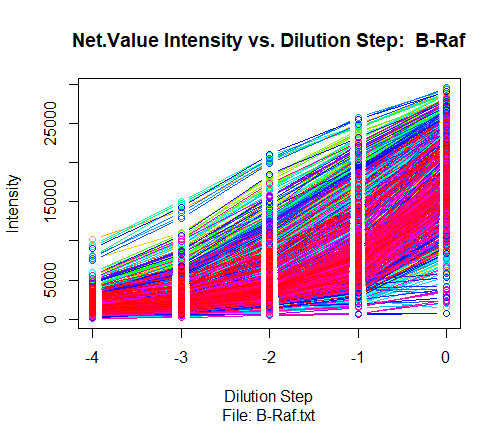
\includegraphics[width=0.49\linewidth]{images/design_check} 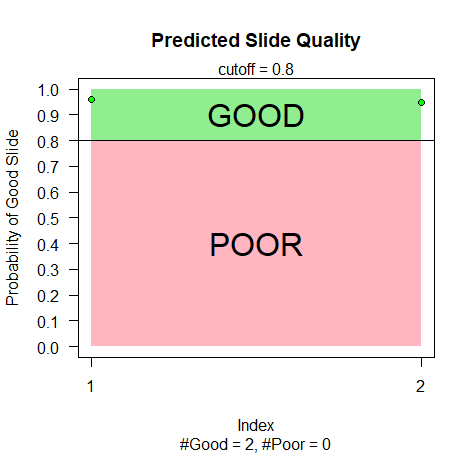
\includegraphics[width=0.49\linewidth]{images/slide_quality} 

}

\caption{Net.Value Intensity vs Dilution Step and Predicted Slide Quality}\label{fig:unnamed-chunk-2}
\end{figure}

The second graph will display if the run of slides is utilizing the
Pre-Fit Quality Control metric like the sample slides do. This will give
an indication of the expected quality of the inputs for the set of
slides and an indicator of the overall number of good and bad slides in
the set.

Neither of the above two graphs are saved to disk. While processing, two
images, each with two graphs will be generated for each of the slides
and saved to disk. These will be displayed on the screen briefly while
the processing occurs. For details of the contents of these graphs, see
the section ``\protect\hyperlink{process_6}{Step 6: Generate Graphical
Output}'' later in this document.

The Run.R process creates a subdirectory named ``out'' in the analysis
directory you specified in step 7 of the previous section. If the slide
sample run ran as expected, there should be 31 output files in that out
directory. For detailed descriptions of each of those files and their
formats see the section ``\protect\hyperlink{outputs}{Outputs and Output
Formats}'' later in this document.

\newpage

\hypertarget{biology}{%
\section{The Biology of RPPAs}\label{biology}}

Reverse Phase Protein Arrays are an antibody-based technique with
procedures similar to that of Western blots. RPPAs resulted from an
attempt to extend the microarray approach to the measurement of
proteins. A microarray is ``forward-phase'' in that it simultaneously
measures the expression levels of many genes in one biological sample.
An RPPA is ``reverse-phase'' in that it simultaneously measures the
expression levels of one protein in many biological samples.

The biological samples of interest are lysed, producing a homogeneous
mixture (lysate), and these lysates are printed onto an array according
to a dilution series. The arrays are typically glass with a
nitrocellulose membrane on one side; the lysates are printed on the
nitrocellulose.

In order to measure the protein of interest, the array is first
interrogated with an antibody specific to the protein of interest (the
primary antibody, typically derived from a mouse, rabbit or goat). This
is allowed to bind, and loose material is washed away. The array is then
interrogated with a labeled antibody (a secondary antibody, such as
anti-goat immunoglobulin) which recognizes the primary antibody. This is
allowed to bind, and loose material is washed away. In the most common
labeling approach, the secondary antibody is linked to an enzyme, as
with enzyme-linked immunosorbent assays (ELISAs). The enzyme substrate
is then introduced. The enzyme reacts with its substrate, causing
precipitate to build up near the site of the reaction: more of the
protein of interest at a spot means more enzyme should bind and more
precipitate should form. After a short period, the loose substrate is
washed away.

After drying, the array is then imaged, typically with a flatbed
scanner, usually producing a TIF image file. (Ideally, the TIF file
should be 16-bit grayscale. We have encountered cases where the files
were exported as true color (24-bit), and then converted to grayscale
afterwards. Depending on the software used, this latter step can
introduce substantial distortions.) The printed spots visible in the
image file are then quantified using software developed for cDNA
microarrays.

Several other methods of labeling the secondary antibody have been
tried, including fluorescent dyes and quantum dots, but all methods
still yield a TIF image file which is then quantified.

\hypertarget{model}{%
\section{The RPPASPACE Model}\label{model}}

A key distinction between reverse-phase and forward-phase assays is that
for reverse-phase assays the hybridization kinetics should be the same
at every spot, as all samples are being queried for the same protein.
Thus, in the case of lysate arrays, we expect there to be a single
common dose-response curve, instead of a separate one for each sample.
In particular, we can borrow strength across samples for the estimation
of baseline and saturation intensity.

We assume that the observed intensity for sample \(i\), dilution step
\(j\), replicate \(k\) can be fit as \[
  y_{ijk} = \alpha + \beta * g(\gamma(\delta_i + x_{ij})) + \epsilon_{ijk},
\] where \(g(x) = e^x/(1+e^x)\).

The shape parameters of the logistic response curve, \(\alpha\),
\(\beta\), and \(\gamma\) are common for all samples. The \(x_{ij}\) are
known offsets from the level of interest, such as the undiluted or
``neat'' state. We typically use \(\log_2\) units for \(x_{ij}\),
letting the adjustment to base \(e\) be subsumed into \(\gamma\). The
\(\delta_i\) terms represent the unknown protein concentration at the
reference level for sample \(i\). Finally, \(\epsilon_{ijk}\) is taken
to be white noise.

We fit the above model using Nonlinear Least Squares nls iteratively,
alternating between fitting the shape parameters and the sample
concentrations.

Although RPPASPACE outputs relative protein concentration values it is
possible to obtain an absolute concentration value if titrates with
known protein concentration are included on the slide to calibrate the
x-axis and map relative values to absolute values.

\hypertarget{vs_supercurve}{%
\section{Differences between RPPASPACE and Its Predecessor,
SuperCurve}\label{vs_supercurve}}

The RPPASPACE R package was developed from the 1.5.15 version of the
SuperCurve R package (see
\url{https://bioinformatics.mdanderson.org/public-software/supercurve/}).

Changes were requested that were not compatible with the existing
codebase of the SuperCurve package. There was also added emphasis on
making the package integrate more easily and provide additional features
for a more comprehensive RPPA processing pipeline known as the RADIAN
Pipeline (see \url{http://www.radianpipeline.org/}). As a result, a new
package was created that eliminated or modified some of the SuperCurve
features, added multiple new features, and enhanced the performance of
the package overall. As a consequence, RPPASPACE is no longer compatible
with the SuperCurve suite of products at
\url{http://r-forge.r-project.org/R/?group_id=1899}.

\textbf{Some of the differences in RPPASPACE 1.0 from its predecessor
SuperCurve include:}

\textbf{New and/or Improved Features:}

\begin{itemize}
\tightlist
\item
  Added code to validate that all slides in a set have the same layout
  and dilution levels for each spot. Skips processing of slide if
  different from the first slide in the set.
\item
  Added option of ``None'' normalization method to allow processing of
  slides without normalization being done by the package.
\item
  Added capability to exclude a list of dilution series from fit curve
  creation without requiring changes to the slide layout.
\item
  Added option to use some or all positive control series as inputs for
  a ``Noise'' QC metric.
\item
  Added support for additional input slide images formats. Now supports
  tif, png, bmp, gif or jpg.
\item
  Added capability to rotate input slide images in 90 degree increments
  if the slide files do not match the orientation of the spots in the
  quantification files.
\end{itemize}

\textbf{Processing Improvements and package updates:}

\begin{itemize}
\tightlist
\item
  Added optional parallelization of some portions of the code for faster
  processing of slide sets.
\item
  Removed dependence of the third-party image processing software
  product ImageMagick.
\item
  Improved error handling. Processing of slide set even if some slides
  fail rather than stopping on the first error.
\item
  Improved error reporting. Outputs error and warning files as part of
  output with more useful error messages for reporting run-time issues.
\item
  Made creation of output jpg optional and not done by default.
\item
  Updated documentation and examples.
\end{itemize}

\textbf{Changes Inputs and Outputs:}

\begin{itemize}
\tightlist
\item
  Switched to a standard slide text input format.
\item
  Eliminated usage of a design file.
\item
  Removed functions related to defining design files or related
  parameters or designing slides without the use of quantification text
  files and removed alias-related functionality.
\item
  Added output file of adjustments made to all slides in set by spatial
  corrections algorithms.
\item
  Added combined QC metrics output file containing QC metrics for all QC
  methods used.
\end{itemize}

\textbf{Bug Fixes and Code Maintenance:}

\begin{itemize}
\tightlist
\item
  Fixed bug causing CobsFitClass to possibly return concentration data
  in wrong order.
\item
  Fixed bug causing spatial correction surface creation to put points on
  wrong surface.
\item
  Added additional package imports for processing: doParallel, foreach,
  parallel, iterators, imager, bmp, jpeg, tiff, png.
\item
  Improved code base - removed unused portions of code in package
  including 8 complete source files and updated some deprecated methods
  in R. Now passes as-cran R CMD check.
\item
  Documented requirement of use of xvfb in headless Unix environments
  for graphics output.
\end{itemize}

\hypertarget{input_data}{%
\section{RPPASPACE Input Data}\label{input_data}}

As mentioned above, the primary data for input into RPPASPACE usually
comes from a multi-step process where an image of a slide has been
created and quantified. Some software products used for the
quantification step include Mapix, MicroVigene, or ArrayPro. The output
of this quantification software will generally be a text file that
usually lists multiple fields that describe the values on the slide.

RPPASPACE requires all slide data to be input into the system in a
specific standardized format. Conversion to this standard text file
format will require custom software/scripts based on the format of the
output of the configuration of quantification software used to quantify
the slide image. Some examples of R scripts used to convert files from
various quantification packages are included in the RPPASPACE package.
Examples can be seen later in this document in the section ``Converting
Slides to Standard Slide Input Format''

RPPASPACE accepts two types of input data:

\begin{itemize}
\tightlist
\item
  Tab-delimited text files with an extension of ``.txt''. (See
  information on the standard slide format below.)
\item
  Optional slide image files in one of the following formats/extensions:
  ``.tif'', ``.png'', ``.bmp'', ``.gif'', or ``.jpg''. It is suggested
  that there only be one slide per image. If the option for creating
  combined output jpg files is utilized, the entire image will be
  appended to graphs created by the RPPASPACE process and output as a
  single jpg output file. If an image for a particular slide is not
  available, then a ``missing image'' graphic file will be appended to
  the output jpg image.
\end{itemize}

In addition to the input data, configuration objects will need to be set
up to run RPPASPACE. This configuration will be detailed in a later
section.

\hypertarget{slide_input_format}{%
\section{RPPASPACE Standard Slide Input
Format}\label{slide_input_format}}

RPPASPACE expects each tab-delimited slide in a set to be in the
following format. There should be a row for each possible spot on the
slide grid mentioned above with the following columns for each row. The
file should contain a header row with the column names listed in the
following table.

\begin{longtable}[]{@{}lll@{}}
\toprule
\begin{minipage}[b]{0.26\columnwidth}\raggedright
Column Name\strut
\end{minipage} & \begin{minipage}[b]{0.26\columnwidth}\raggedright
R Data Type\strut
\end{minipage} & \begin{minipage}[b]{0.40\columnwidth}\raggedright
Description\strut
\end{minipage}\tabularnewline
\midrule
\endhead
\begin{minipage}[t]{0.26\columnwidth}\raggedright
Order\strut
\end{minipage} & \begin{minipage}[t]{0.26\columnwidth}\raggedright
Integer\strut
\end{minipage} & \begin{minipage}[t]{0.40\columnwidth}\raggedright
Order of the points in this file. Used for tracking/error reporting.
Generally expected to be 1 through number of points on the slide.\strut
\end{minipage}\tabularnewline
\begin{minipage}[t]{0.26\columnwidth}\raggedright
Main.Row\strut
\end{minipage} & \begin{minipage}[t]{0.26\columnwidth}\raggedright
Integer\strut
\end{minipage} & \begin{minipage}[t]{0.40\columnwidth}\raggedright
Main grid row number\strut
\end{minipage}\tabularnewline
\begin{minipage}[t]{0.26\columnwidth}\raggedright
Main.Col\strut
\end{minipage} & \begin{minipage}[t]{0.26\columnwidth}\raggedright
Integer\strut
\end{minipage} & \begin{minipage}[t]{0.40\columnwidth}\raggedright
Main grid column number\strut
\end{minipage}\tabularnewline
\begin{minipage}[t]{0.26\columnwidth}\raggedright
Sub.Row\strut
\end{minipage} & \begin{minipage}[t]{0.26\columnwidth}\raggedright
Integer\strut
\end{minipage} & \begin{minipage}[t]{0.40\columnwidth}\raggedright
Sub grid row number\strut
\end{minipage}\tabularnewline
\begin{minipage}[t]{0.26\columnwidth}\raggedright
Sub.Col\strut
\end{minipage} & \begin{minipage}[t]{0.26\columnwidth}\raggedright
Integer\strut
\end{minipage} & \begin{minipage}[t]{0.40\columnwidth}\raggedright
Sub grid column number\strut
\end{minipage}\tabularnewline
\begin{minipage}[t]{0.26\columnwidth}\raggedright
Series.Id\strut
\end{minipage} & \begin{minipage}[t]{0.26\columnwidth}\raggedright
Integer\strut
\end{minipage} & \begin{minipage}[t]{0.40\columnwidth}\raggedright
0 for Blank spots and negative controls, Integer from 1 to number of
sample dilution series printed on the slide. Additional integer values
for positive controls series if those are used.\strut
\end{minipage}\tabularnewline
\begin{minipage}[t]{0.26\columnwidth}\raggedright
Spot.Type\strut
\end{minipage} & \begin{minipage}[t]{0.26\columnwidth}\raggedright
String\strut
\end{minipage} & \begin{minipage}[t]{0.40\columnwidth}\raggedright
Case-insensitive text string describing the type of spot at this grid
location. Only one spot type is allowed per spot. Acceptable values
include: ``Sample'', ``Blank'', ``Buffer'', ``NegCtrl'', ``PosCtrl'',
``PosCtrl-Noise'', and ``Noise''. For many labs, the only values that
would be likely to be needed would be ``Sample'' and possibly
``Blank''.\strut
\end{minipage}\tabularnewline
\begin{minipage}[t]{0.26\columnwidth}\raggedright
Dilution\strut
\end{minipage} & \begin{minipage}[t]{0.26\columnwidth}\raggedright
Double\strut
\end{minipage} & \begin{minipage}[t]{0.40\columnwidth}\raggedright
The decimal value of the dilution, or 0 for blank areas and negative
control points. Common 2-fold values would be a subset of: 100, 50, 25,
12.5, 6.25, 3.125, 1.5625, and 0.78125.\strut
\end{minipage}\tabularnewline
\begin{minipage}[t]{0.26\columnwidth}\raggedright
Net.Value\strut
\end{minipage} & \begin{minipage}[t]{0.26\columnwidth}\raggedright
Double\strut
\end{minipage} & \begin{minipage}[t]{0.40\columnwidth}\raggedright
The value of the spot calculated by subtracting the Background.Value
from the Raw.Value\strut
\end{minipage}\tabularnewline
\begin{minipage}[t]{0.26\columnwidth}\raggedright
Background.Value\strut
\end{minipage} & \begin{minipage}[t]{0.26\columnwidth}\raggedright
Double\strut
\end{minipage} & \begin{minipage}[t]{0.40\columnwidth}\raggedright
The value of the background around the spot (usually mean value of
pixels) in 16 bit value.\strut
\end{minipage}\tabularnewline
\begin{minipage}[t]{0.26\columnwidth}\raggedright
Spot.X.Position\strut
\end{minipage} & \begin{minipage}[t]{0.26\columnwidth}\raggedright
Double\strut
\end{minipage} & \begin{minipage}[t]{0.40\columnwidth}\raggedright
Horizontal position (in pixels) of center of spot on image. Not actually
used in RPPASPACE software, but can be used when debugging to help
locate the spot in the original image.\strut
\end{minipage}\tabularnewline
\begin{minipage}[t]{0.26\columnwidth}\raggedright
Spot.Y.Position\strut
\end{minipage} & \begin{minipage}[t]{0.26\columnwidth}\raggedright
Double\strut
\end{minipage} & \begin{minipage}[t]{0.40\columnwidth}\raggedright
Vertical position (in pixels) of center of spot on image. Not actually
used in RPPASPACE software, but can be used when debugging to help
locate the spot in the original image.\strut
\end{minipage}\tabularnewline
\begin{minipage}[t]{0.26\columnwidth}\raggedright
Original.Order\strut
\end{minipage} & \begin{minipage}[t]{0.26\columnwidth}\raggedright
Numeric\strut
\end{minipage} & \begin{minipage}[t]{0.40\columnwidth}\raggedright
The original order of the spots in the source file before conversion.
This should be created by user's slide conversion script outside of
RPPASPACE. (Useful for tracking back to the original quantified values
if there is a problems on a slide. Not actually used by RPPASPACE for
processing.)\strut
\end{minipage}\tabularnewline
\begin{minipage}[t]{0.26\columnwidth}\raggedright
\strut
\end{minipage} & \begin{minipage}[t]{0.26\columnwidth}\raggedright
\strut
\end{minipage} & \begin{minipage}[t]{0.40\columnwidth}\raggedright
\strut
\end{minipage}\tabularnewline
\bottomrule
\end{longtable}

\hypertarget{expectations}{%
\section{RPPASPACE Expectations of Input Data}\label{expectations}}

\begin{enumerate}
\def\labelenumi{\arabic{enumi})}
\tightlist
\item
  All slide input data will be in text files in the standard slide input
  format specified above. These will be referred to as the slide
  quantification text files in later descriptions in this document.
\item
  Each slide quantification text file should contain information for
  only one slide.
\item
  All slide quantification text files for a RPPASPACE run will be in one
  directory.
\item
  All slide quantification text files for a RPPASPACE run will have the
  same slide layout. (First 8 columns of each slide in set should be
  identical.)
\item
  The spots on each slide will be laid out in a regularly spaced
  rectangular grid pattern of rows and columns.\\
\item
  If the layout of the slide is not broken into obvious subgrids, then
  the Main.Row and Main.Col fields in the input file can all be set to 1
  with the Sub.Row and Sub.Col representing the location in the overall
  grid.
\item
  Each slide will consist of multiple sample dilution series, assigned a
  series id that is a positive integer from 1 to the number of series on
  the slide.
\item
  Biological or technical replicates of a series should be treated as
  separate series and assigned a unique series number.
\item
  Series dilutions levels will have a high value of 100 and a low value
  greater than zero.
\item
  All dilution series that are on a slide will have the same number of
  dilution points.
\item
  All dilution series on a slide will include one and only one spot for
  each dilution level.
\item
  If included, positive controls and their two noise variations, will
  also be dilution series, with the same number of points and same
  dilution levels as the sample series on the slide and will be assigned
  a series id in the same manner as the sample dilution series.
\item
  Each slide may optionally have negative control points or blank spots
  in the grid.
\item
  If negative controls are included on the slide they will all have a
  dilution of 0 and a series id of 0.
\item
  If positive controls or noise controls are present on the slide,
  negative controls must also be present if spatial corrections, pre-fit
  QC , and/or noise calculations are to be calculated as part of the
  processing of the slide set.
\item
  If images of the original slides are to be included in the output, all
  input slide images for a run must be of the same file type (with a
  common file extension) and stored in the same directory. Slide file
  names (excluding the file extension) must match the file names of the
  slide input text files for the run. Files not matching one of the
  slide names will be ignored. All slide image files are optional. These
  will only be used for creating a final output jpg image for each
  processed slide. If no image of the designated format is present for a
  given slide a ``missing image'' graphic will be included in the final
  output jpg image.
\item
  Any spot in the rectangular grid that should always be ignored during
  processing should be assigned a Spot.Type of ``Blank'' and should have
  a dilution of 0 and a Series.Id of 0.
\end{enumerate}

\hypertarget{controls}{%
\section{Positive and Negative Controls}\label{controls}}

RPPASPACE uses the Net.Value column of the input slide for its
calculations. As the Net.Value is expected to be the difference between
the Raw.Value and the Background.Value for each spot, variations in the
background of the slide can cause variations in the intensities of the
spots used in the calculations. If the background were uniform, then
spots with nothing, or just a buffer solution printed on them (negative
controls) should have the same values across the slide. In addition,
replicates of a single dilution series (positive controls) printed at
various positions on the slide should also have consistent values at
each dilution level.

If such positive and negative controls are spread out in a regular
fashion across a slide, the RPPASPACE package provides mechanisms for
judging the quality of the slide (known as the pre-fit QC value) before
doing further processing, and for adjusting the values of the sample
points in a manner to correct for the regional differences in the
positive control points in the region around each sample (spatial
correction).

For best accuracy, it is suggested that slides utilizing the pre-fit QC
calculations or spatial corrections divide the slide into rectangular
subgrids and place at least one negative control and one or more
positive control series in each subgrid of the slide.

\hypertarget{layout_example}{%
\section{Slide Layout Example}\label{layout_example}}

In the MD Anderson RPPA Lab, slides are laid out in a regular
rectangular grid consisting of 5808 spots, 132 spots in the horizontal
direction and 44 spots in the vertical direction, with a label area on
the right side of the slide, as seen in the figure below ``Example MD
Anderson Slide Image''.

\begin{figure}

{\centering 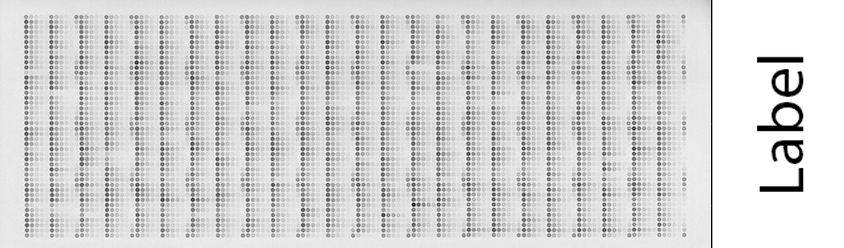
\includegraphics[width=0.9\linewidth]{images/example_slide} 

}

\caption{Example MD Anderson Slide Image}\label{fig:unnamed-chunk-3}
\end{figure}

The slide shown above can be subdivided into subgrids of 11 spots by 11
spots with 12 subgrids horizontally and 4 subgrids vertically as shown
in the figure below ``MD Anderson Slide Layout Showing Subgrids''.

\begin{figure}

{\centering 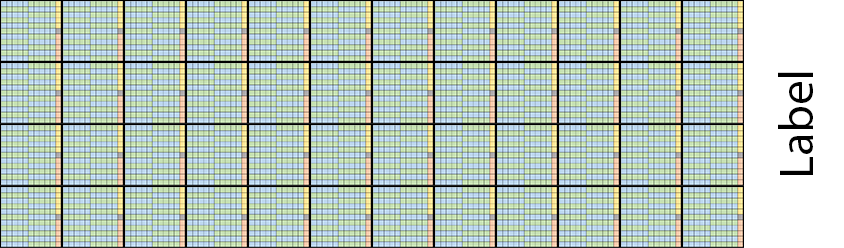
\includegraphics[width=0.9\linewidth]{images/example_slide_with_subgrids} 

}

\caption{MD Anderson Slide Layout Showing Subgrids}\label{fig:unnamed-chunk-4}
\end{figure}

Subgrids can be a useful way of helping to organize the layout of the
samples and control points on a slide. In SuperCurve, the subgrids could
be used along with the design file to determine what order the data in
the input file might be processed. Since the input file specification in
RPPASPACE utilizes a common layout, the subgrids now mainly serve as an
optional method for managing the layout of an input slide.

In the standard MDA format, one subgrid would contain 11 spots
horizontally by 11 spots vertically.

\begin{figure}

{\centering 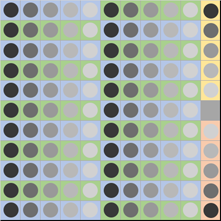
\includegraphics[width=0.3\linewidth]{images/single_subgrid} 

}

\caption{Example of Single Subgrid Layout}\label{fig:unnamed-chunk-5}
\end{figure}

In the example subgrid layout shown in the figure, ``Example of Single
Subgrid Layout'', the backgrounds of each square are color-coded to help
explain the function of each part of the subgrid. The squares with blue
and green backgrounds are 5-spot dilution series representing samples
for which RPPASPACE tries to calculate the relative concentrations. Ten
squares along the right side represent two copies of 5-spot positive
control dilution series. The grey square on the center of the right side
(11th column) is a negative control spot.

Two-fold dilution series for samples on slides in the standard MDA
format are printed horizontally with the highest concentration on the
left and decreasing toward the right. Positive and negative control
spots are arranged such that within each subgrid, the first copy of the
positive control series starts at the top, ~decreasing vertically. Below
the first series is a negative control spot, followed by another copy of
the positive control series, starting with the lowest concentration and
increasing to the highest concentration. Points could actually be
anywhere on the grid as long as they are consistent between slides in a
set being processed.

Within the quantification text file representing the slide values, each
spot on the slide would be represented by one row. As described in The
Spot.Type column would contain ``Sample'', ``PosCtrl'', and ``NegCtrl''
respectively for the samples, positive controls, and negative controls.
This pattern is repeated for each subgrid of the slide.

\hypertarget{replicated_series}{%
\section{Handling of Replicated Sample Dilution
Series}\label{replicated_series}}

Some labs print replicated dilution series of the same samples on a
single slide and combine the repeated samples in some manner, such as
taking the mean of the spots for each dilution level. RPPASPACE expects
all dilution series on a slide to have the same number of points and for
no dilutions to be repeated within a series. When using RPPASPACE,
replicated series on the slide should be treated as separate samples
with different Series.Id values. Any processing to combine the
replicated series should either be done before the slide is passed to
RPPASPACE to process or be combined after the RPPASPACE process has
completed.

\hypertarget{missing_series}{%
\section{Support of Missing or Skipped Sample
Series}\label{missing_series}}

Some labs we have worked with may have a rectangular grid of spots, but
may skip some series for some reason such as leaving a blank area
between samples from different sources, or may know that some spots on a
particular set were not valid and just want to skip processing them. The
best way to handle these skipped spots is to mark them as ``Blank'' in
the quantification text files when converting them to the standardized
format used by RPPASPACE. This will cause the spots to not be used in
calculating the concentration curve and to not plot those points on the
output plots.

If you just want to skip some sample series from being used to calculate
the concentration curve, but still want those samples to be plotted on
the output graphs, then RPPASPACE provides a way to specify which
samples to ignore when calculating the curves for the slides in the set.
Create a list of the Sample.Id values for the samples to be excluded
from the curve calculations and assign that list to the seriesToIgnore
parameter of the RPPADesignParameters class when configuring RPPASPACE.

\hypertarget{random_order}{%
\section{Randomly Ordered Slides}\label{random_order}}

The standard slide format used in the MD Anderson RPPA Lab prints the
spots for each sample dilution series near one another so that it is
easier to do a visual inspection of the slide to get an idea of how well
the printing and staining process went. This is not a requirement of the
RPPASPACE software. Spots can appear in any order in the grid as long as
they are properly designated in the quantification text input file. All
slides in a set must follow the same ordering.

\hypertarget{process}{%
\section{The RPPASPACE Process}\label{process}}

RPPASPACE processes a set of slides as follows:\\
1. \protect\hyperlink{process_1}{Read a set of slide quantification
files from a specified directory.}\\
2. \protect\hyperlink{process_2}{Perform pre-fit quality assurance
checks. (optional).}\\
3. \protect\hyperlink{process_3}{Perform spatial adjustments
(optional).}\\
4. \protect\hyperlink{process_4}{Perform curve fitting and calculate
relative concentrations.}\\
5. \protect\hyperlink{process_5}{Perform noise quality control
calculations (optional).}\\
6. \protect\hyperlink{process_6}{Generate graphical output.}\\
7. \protect\hyperlink{process_7}{Slide Normalization.}\\
8. \protect\hyperlink{process_8}{Write final results.}

\hypertarget{process_1}{%
\subsection{Read Slide Quantification Files}\label{process_1}}

As part of the setup process, the user supplies a directory containing
the set of quantification text files representing RPPA slides. It is
expected that each quantification file representing a slide is named
with the name of the antibody used on the slide and an extension of
``.txt''. The software gathers a list of all files in that directory
with a ``.txt'' file extension. The contents of the first file found
will be used to determine the expected layout of all of the slides in
that set. The columns compared include Order, Main.Row, Main.Col,
Sub.Row, Sub.Col, Series.Id, Spot.Type, and Dilution. Each text file
that doesn't have the same values with respect to those columns will
generate an error message and will not be processed by the following
steps of the process.

The name of the file, without the .txt extension, will be used as the
name of the antibody/slide being processed. Additional steps in the
process will use the file name when referring to that slide when
reporting errors and providing the final output. Internally, each file
will be used to construct a RPPA object and the set of all the RPPA
objects to be processed will be part of an RPPASet object.

Specification of the input directory for the quantification files is
done by setting the txtdir parameter of the RPPASPACESettings object of
the RPPASPACE package.

If there are issues in reading the data for a particular slide or all
slides in general, then messages regarding the issues will be written to
the designated error output file.

\hypertarget{process_2}{%
\subsection{Perform Pre-Fit Quality Assurance Check}\label{process_2}}

The RPPASPACE package includes methods to provide a quality assurance
check under the following conditions:\\
. The parameter doprefitqc has been set to true in the RPPASettings
configuration object.\\
. The appropriate positive and negative controls have been included as
part of the slides.\\
. The slides use 5 point dilution series. For slides with dilution
series with some other number of dilution points, the Pre-Fit Quality
Assurance Step will be skipped.

If these conditions are met, the Pre-Fit Quality Assurance (Prefit-QC)
code will be run to calculate a value between 0 (bad) and 1 (good) to
indicate the quality of each slide. Typically, we treat any value below
.8 as indicating a bad slide that probably needs to be reprocessed or
removed from the set. Output from this routine will be written to a file
named ``rppaspace\_prefit\_qc.csv'' in the specified output directory.

Specific details of the configuration parameters for the pre-fit QC
portions of the RPPASPACE process can be found in the help for the
doprefitqc and onlynormqcgood parameters of the RPPASPACESettings object
of the RPPASPACE package.

The calculations are based on a number of features of the slide. For a
more technical description on the methods used by RPPASPACE to perform
Quality control checks see the paper
``\href{https://www.ncbi.nlm.nih.gov/pmc/articles/PMC4375399/}{Development
of a robust classifier for quality control of reverse-phase protein
arrays}''.

If there are issues in computing the pre-fit quality control values for
a particular slide or all slides in general, then messages regarding the
issues will be written to the designated warning or error output file,
depending on the severity of the issue.

\hypertarget{process_3}{%
\subsection{Perform Spatial Adjustments}\label{process_3}}

For multiple reasons, background and foreground intensities may vary
across the surface of a slide. RPPASPACE offers a method of correcting
for such variations if the slides are properly configured. For this
method to work, multiple dilution series of a common substance (known as
positive controls) must be printed across the slide in a regular
grid-like pattern. If a slide did not have background and foreground
variations, one would expect such replicated positive control dilution
series on the slide to all have nearly identical values at each dilution
level. If these values do differ, then it can be assumed that values of
samples between these replicates may vary in a similar manner and can be
used to adjust the values of the samples. As background noise inherent
in the slide creation process may be larger than some of the values of
the spots of some lower intensities, negative controls (spots with
nothing or only a buffer substance printed on the slide) are used to
determine a low cutoff point at which the positive controls will be
ignored when calculating the spatial corrections.

If spatial correction is requested for the run of RPPASPACE, spatial
adjustments are performed on each slide individually and the values used
to adjust each spot on each slide will be written to the output
directory in a single file named ``spatial\_adjustments.tsv''. The tab
separated file will contain a column for each slide in the set of slides
and a row for each point on the slide. Unlike the other text-based
output files, the spatial corrections file will be written to disk as
soon as the spatial corrections have been calculated for all slides.

If errors are generated while calculating the spatial adjustments for a
slide, then later calculations such as curve fitting and graphics output
will use the original data for that slide rather than the spatially
corrected data for that slide. Slides that were not spatially corrected
due to errors will contain a column of all 0's for those slides due to
their not being adjusted for later calculations.

Specific details of the configuration parameters for the spatial
corrections portions of the RPPASPACE process can be found in the help
for the RPPASpatialParams object of the RPPASPACE package.

Some of the positive control series on a set of slides may be treated
differently than others dependent on the Spot.Type field setting. See
the section ``Perform Noise Quality Control Calculations'' below for
more information on this option.

For a more technical description on the methods used by RPPASPACE to
perform spatial corrections, see the paper
``\href{https://www.ncbi.nlm.nih.gov/pmc/articles/PMC4264691/}{Spatial
Normalization of Reverse Phase Protein Array Data}''.

If there are issues in computing the spatial adjustments values for a
particular slide or all slides in general, then messages regarding the
issues will be written to the designated warning or error output file,
dependent on the severity of the issue.

\hypertarget{process_4}{%
\subsection{Perform Curve Fitting and Calculate Relative
Concentrations}\label{process_4}}

One of the major goals in RPPASPACE is to create a model based on the
intensity values of the spots on a slide of input data and use the model
to provide a computed relative concentration for each sample dilution
series on the slide. Multiple algorithms are available in RPPASPACE for
creating the model of the input data including logistic, loess (Local
Polynomial Regression), and COBS (a monotone increasing B-Spline). See
\url{https://cran.r-project.org/web/packages/cobs/} for technical
details on the R COBS package. RPPASPACE provides mechanisms to allow
users to register other custom models using the registerModel function.

By default, a model is created using all of the points of all of the
samples on an individual slide. As described in the introduction, the
generated curve of intensity values vs log concentration values is
expected to generate a curve for each slide that is sigmoidal in shape.
The midpoint of the high and low intensities for each sample is
calculated and are used as inputs into the model to calculate the
estimated concentration for that sample along that sigmoidal curve. This
is referred to as the EC50 for a sample. The EC50 values for all slides
in the set are written to a comma separated value file in the output
directory named ``rppaspace\_conc\_raw.csv''. This file will have a
column for each slide in the set of slides and a row for each sample.

As mentioned above, by default, all dilution series marked as samples in
the input slide are used for creating the model. RPPASPACE provides a
mechanism to ignore some samples on the slides for a given set of slides
when fitting the curve to the input data. Each sample is assigned a
Sample.Id in the input quantification files. To exclude samples when
constructing the model, the Sample.Ids of the samples to skip to exclude
are added to a list and that list is assigned to the seriesToIgnore
parameter of RPPADesignParams object. These samples will not be used to
construct the model, but will still be fit to the curve and output as
they would normally be by RPPASPACE.

Specific details of the configuration parameters for the curve fitting
and concentration calculation portions of the RPPASPACE process can be
found in the help for the RPPADesignParams and RPPAFitParams objects of
the RPPASPACE package.

For a more technical description on the methods used by RPPASPACE to
perform curve fitting and the overall theory of the process, see the
paper
``\href{https://academic.oup.com/bioinformatics/article/23/15/1986/205819}{Non-parametric
quantification of protein lysate arrays}''.

Users can also add their own curve fitting methods to the process by
registering their methods with the RPPASPACE system. See the help for
the registerModel function for more information.

If there are issues in creating or fitting the curve for a particular
slide or all slides in general, then messages regarding the issues will
be written to the designated warning or error output file, depending on
the severity of the issue.

\hypertarget{process_5}{%
\subsection{Perform Noise Quality Control
Calculations}\label{process_5}}

If positive and negative controls are part of the slide layout, an
additional QC metric, called the Noise Quality Control metric, is
available for calculation. Instead of using all of the positive control
dilution series only as positive controls, some can be alternately used
to calculate the new metric. This is done by setting the Spot.Type
fields in the slide quantification files for a set of slides for some of
the positive control series to either Noise or PosCtrl-Noise instead of
PosCtrl. The Spot.Type designation will determine how those spots are
treated when processing the slides.

The dilution series is treated as follows, depending on the Spot.Type
chosen for that dilution series.

\textbf{Spot.Type = PosCtrl}

\begin{itemize}
\tightlist
\item
  Will be used in Pre-fit QC Metric calculations.
\item
  Will be used in spatial correction calculations.
\item
  Spatial Correction results will not be applied to these points.
\item
  Will not be used to calculate the curve for the slide.
\item
  Will not be fit to the curve for the slide nor used in the Noise QC
  metric.
\end{itemize}

\textbf{Spot.Type = PosCtrl-Noise}

\begin{itemize}
\tightlist
\item
  Will be used in Pre-fit QC Metric calculations.
\item
  Will be used in spatial correction calculations.
\item
  Spatial Correction results will be applied to these points.
\item
  Will not be used to calculate the curve for the slide.
\item
  Will be fit to the curve for the slide used in the Noise QC metric.
\end{itemize}

\textbf{Spot.Type = Noise}

\begin{itemize}
\tightlist
\item
  Will be used in Pre-fit QC Metric calculations.
\item
  Will not be used in spatial correction calculations.
\item
  Spatial Correction results will be applied to these points.
\item
  Will not be used to calculate the curve for the slide.
\item
  Will be fit to the curve for the slide and used in the Noise QC
  metric.
\end{itemize}

If any of the dilution series in a slide file are marked as either Noise
or PosCtrl-Noise, then the Noise QC metric will be calculated for the
set of slides and written to the files ``rppaspace\_noise.csv'' and
``rppaspace\_combined\_qc.csv'' in the output directory.

The dilution series designated as Noise or PosCtrl-Noise series will be
treated similarly to the sample points on the slide. They will be used
calculate a logistic curve for all of the Noise series. Slopes between
consecutive points of the noise dilution series along that curve will be
calculated and any slopes below 0.001 will not be used later noise
calculations. For the remaining points, concentrations for the noise
dilution series are estimated using the same curve generated for the
sample points on the slide as described in the previous section
``Perform Curve Fitting and Calculate Relative Concentrations''. The
calculated concentration values are output as the Noise QC metric values
for these dilution series and are also plotted on the plots described in
the section ``Generate Graphical Output''.

If there are issues in calculating the noise statistics for a particular
slide or all slides in general, then messages regarding the issues will
be written to the designated warning or error output file, depending on
the severity of the issue.

\hypertarget{process_6}{%
\subsection{Generate Graphical Output}\label{process_6}}

For each slide that was successfully processed by RPPASPACE, two
graphics files are created in the output directory that each contain two
plots. The two png files output for the slide will be named with a
prefix of ``rppaspace\_'' followed by the antibody name for the
corresponding slide followed by "\_1.png" or "\_2.png``. Each contain
two plots, as shown in figures below,''Sample PNG \#1" and ``Sample PNG
\#2''.

\begin{figure}
\centering
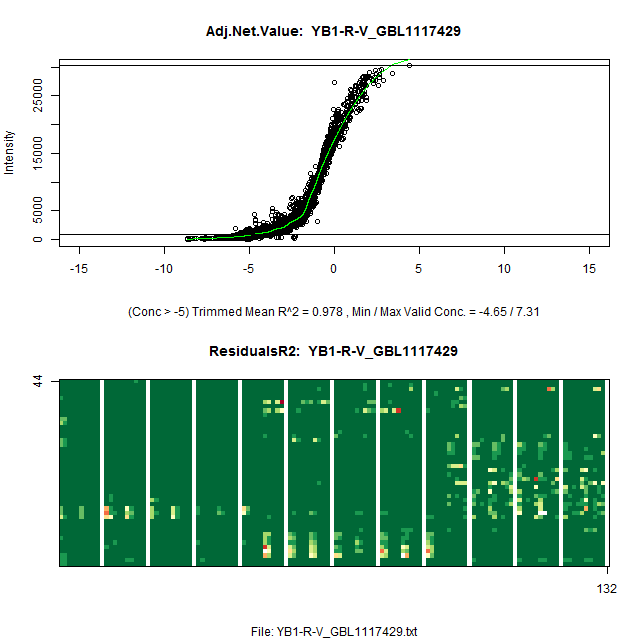
\includegraphics{images/sample_png_1.png}
\caption{Sample PNG \#1}
\end{figure}

Sample PNG \# 1 consists of two graphs. The top graph is a 2 dimension
points plot of the input intensities (modified by spatial adjustments,
if appropriate) along the y axis and the calculated log 2 concentrations
along the x axis. The green line displays the curve modeled by the
selected curve fitting method. The second graph provides a geographic
plot of some measure computed from the fit. The default is to image the
(raw) residuals, with options for other forms of the residuals or for
the fitted concentrations (X) or intensities (Y). Residuals options
include residuals (``Residuals''), standardized residuals (``StdRes''),
r2 residuals (``ResidualsR2''), fitted x (``X''), and fitted y (``Y'').
In this plot there is one square for each point on the slide. Blocks are
dark green where residuals are near zero. The solid white columns in
Figure 4 above represent the positive and negative control points on the
slide.

\begin{figure}
\centering
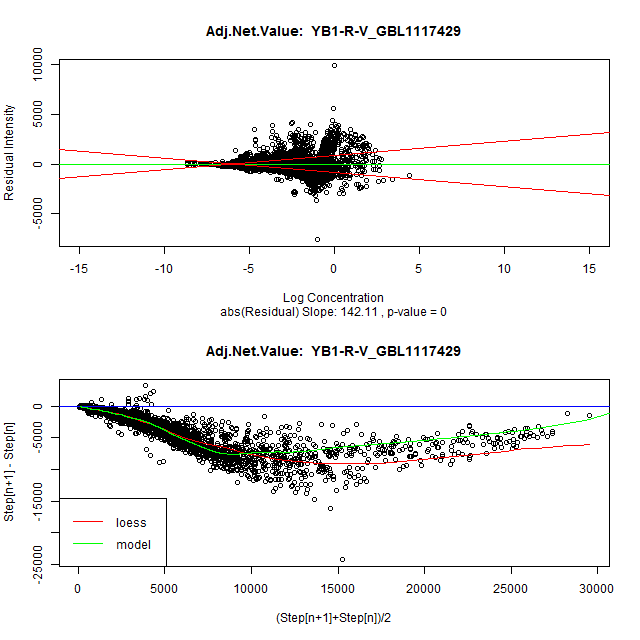
\includegraphics{images/sample_png_2.png}
\caption{Figure 5: Sample PNG \#2}
\end{figure}

Sample PNG \# 2 also consists of two graphs. The top graph is a plot of
the residuals vs.~estimated concentration and can be used to check for
heteroscedasticity. A model of absolute residual values vs.~estimated
concentration is created to assist in doing a rough check for increasing
heteroscedasticity and is displayed as red lines on the graph. A green
horizontal line is drawn through the center of the model points. The
second graph displays a plot for each sample of the difference between
adjacent points in a sample dilution versus the average of those two
points. Plots of the loess (in red) and selected model (in green), in
this example the using the COBS curve fitting method, over the same data
are displayed to assist in determining how well the respective models
fit the sample data.

If an output jpg file is requested, then a jpg file will also be created
for each slide that will be a combination of the two png files and a
scaled down version of the original slide image file, if one is
provided. The software will search for images in the directory specified
by the user in the imgdir parameter of the RPPASPACESettings object
specified by the user when running RPPASPACE. The software will search
for image files with the extension as specified in the imageextension
parameter of the same object. If no imageextension parameter is provided
then the software will default to searching for files with the extension
``.tif''. Supported file types and extensions include ``.tif'',
``.png'', ``.bmp'', ``.gif'', and ``.jpg''. All image files for a set of
slides must be of the same image type with the specified file extension.
The portion of the file name without the file extension will be compared
to the antibody names from the input quantification files. Where there
is not an exact match of the file name with the expected image
extension, then a default image labeled ``missing slide image'' will be
shown where the scaled slide image would normally appear in the output
jpg file. The output jpg file will be named with the antibody name of
the input slide quantification file. If there are issues in generating
graphics for a particular slide or all slides in general, then messages
regarding the issues will be written to the designated warning or error
output file, depending on the severity of the issue.

\newpage

\hypertarget{process_7}{%
\subsection{Slide Normalization}\label{process_7}}

RPPASPACE inherits the functionality of the SuperCurve package for
normalizing slides for slide-to-slide quantification differences across
a set of slides. The RPPASPACE package requires the user to select a
normalization method and will output normalized slide data based on the
method selected. A text file with a name formatted as
rppaspace\_{[}normalization method{]} will be written to the output
directory.

RPPASPACE is designed to support the following normalization methods:
Median Polish (medpolish), Median (median), Housekeeping (house),
Variable Slope (vs), and None (none)

\begin{longtable}[]{@{}ll@{}}
\toprule
\begin{minipage}[b]{0.37\columnwidth}\raggedright
Method\strut
\end{minipage} & \begin{minipage}[b]{0.57\columnwidth}\raggedright
Description\strut
\end{minipage}\tabularnewline
\midrule
\endhead
\begin{minipage}[t]{0.37\columnwidth}\raggedright
Median Polish\strut
\end{minipage} & \begin{minipage}[t]{0.57\columnwidth}\raggedright
Fits additive model using Tukey's median polish.\strut
\end{minipage}\tabularnewline
\begin{minipage}[t]{0.37\columnwidth}\raggedright
Median\strut
\end{minipage} & \begin{minipage}[t]{0.57\columnwidth}\raggedright
Sample median is subtracted from each sample.\strut
\end{minipage}\tabularnewline
\begin{minipage}[t]{0.37\columnwidth}\raggedright
Housekeeping\strut
\end{minipage} & \begin{minipage}[t]{0.57\columnwidth}\raggedright
Median of set of housekeeping antibodies is subtracted from each
sample.\strut
\end{minipage}\tabularnewline
\begin{minipage}[t]{0.37\columnwidth}\raggedright
Variable Slope\strut
\end{minipage} & \begin{minipage}[t]{0.57\columnwidth}\raggedright
Sample median is subtracted from each sample after applying
multiplicative gamma. For a more technical description on variable slope
normalization, see the paper
\href{http://dx.doi.org/10.1093/bioinformatics/btp174}{``Variable Slope
Normalization of Reverse Phase Protein Arrays''}\strut
\end{minipage}\tabularnewline
\begin{minipage}[t]{0.37\columnwidth}\raggedright
None\strut
\end{minipage} & \begin{minipage}[t]{0.57\columnwidth}\raggedright
RPPASPACE was designed to work better with the new RADIAN pipeline being
created at MD Anderson for processing RPPA sets. This pipeline has its
own methods of slide normalization, so preforming extra calculations
within RPPASPACE would not provide additional benefit but would take
additional time. As a result, an additional method of ``none'' was added
to the existing normalization methods to skip doing extra calculations
as part of the RPPASPACE process.\strut
\end{minipage}\tabularnewline
\begin{minipage}[t]{0.37\columnwidth}\raggedright
\strut
\end{minipage} & \begin{minipage}[t]{0.57\columnwidth}\raggedright
\strut
\end{minipage}\tabularnewline
\bottomrule
\end{longtable}

Users can also add their own normalization methods to the process by
registering their methods with the RPPASPACE system. See the help for
the registerNormalizationMethod function for more information.

If there are issues in slide normalization for a particular slide or all
slides in general, then messages regarding the issues will be written to
the designated warning or error output file, depending on the severity
of the issue.

\hypertarget{process_8}{%
\subsection{Write Final Results}\label{process_8}}

Multiple text files representing the results of the previous steps are
written to the output directory after the graphics output step is
complete. For more information on the specifics of the output files, see
the individual sections above and the section on
``\protect\hyperlink{outputs}{Outputs and Output Formats}'' below.

If there are issues in outputting the results for a particular slide or
all slides in general for any of these output files, then messages
regarding the issues will be written to the designated warning or error
output file, depending on the severity of the issue.

\hypertarget{using_rppaspace}{%
\section{Using RPPASPACE}\label{using_rppaspace}}

Using RPPASPACE consists of a few steps: setting up your R environment
with the prerequisite packages, formatting and organizing your input
data, creating a Settings object to tell where to find and how to
process your input data and where outputs should be written, and calling
the fitCurveAndSummarizeFromSettings function in RPPASPACE to start the
process.

\hypertarget{r_env}{%
\section{Setting Up Your R Environment}\label{r_env}}

As described in the RPPASPACE package description file, RPPASPACE
requires an R version greater than or equal to 2.5 and utilizes the
following packages:\\
\textbf{Requires}: methods, doParallel, foreach, parallel, iterators\\
\textbf{Imports}: utils, grDevices, graphics, stats, MASS, cobs,
magrittr, imager, bmp, jpeg, tiff, png\\
\textbf{Suggests}: boot, mgcv, quantreg, robustbase, splines, timeDate

It is best to have all of the above packages installed on your system
before trying to use RPPASPACE.

\hypertarget{formatting_inputs}{%
\section{Organizing and Formatting Of Input
Data}\label{formatting_inputs}}

As mentioned in earlier sections, RPPASPACE inputs two types of data,
slide quantification files and optionally, slide image files for each
slide. RPPASPACE processes slides in a slide set. A slide set consists
of one or more slide quantification text files and optional associated
image files. It is expected that all slide quantification files for a
given set will reside in a single directory. Also, all images for a
specific set will reside in a single directory. File names for both
images and quantification files, minus the final file extensions, must
be identical for the image file to be matched with a corresponding
slide.

Details on the expected input file formats supported can be found in the
sections above labelled ``\protect\hyperlink{input_data}{RPPASPACE Input
Data}'', ``\protect\hyperlink{slide_input_format}{RPPASPACE Standard
Slide Input Format}'', and ``\protect\hyperlink{expectations}{RPPASPACE
Expectations of Input Data}''. A sample R script for converting data
from an ARRAYPRO (used at MD Anderson) input formats can be found in the
inst/sampleCode directory of the RPPASPACE package. See section
``\protect\hyperlink{converting}{Converting Slides To Standard Slide
Input Format}'' for additional information on how to convert your lab's
slides for use in RPPASPACE.

\hypertarget{settings}{%
\section{Creating an RPPASPACESettings Object}\label{settings}}

The RPPASPACESettings object is part of the RPPASPACE package. It is
used to define directory paths and image file type specifiers for input
data, directory paths and file names for output data, and parameters
containing other RPPASPACE objects that specify which features of the
package are to be used in processing the data.

See the package help for full details on this object and the defaults
for the calling parameters as well as specifics of the other objects
provided by the RPPASPACE package used by the RPPASPACESettings object.
These include RPPADesignParams, OptionalRPPASpatialParams,
RPPAFitParams, and RPPANormalizationParams objects.

\hypertarget{example_script}{%
\section{Example RPPASPACE Script}\label{example_script}}

Note: a copy of the following script file, with some additional minor
output but with fewer comments, exists in the inst/sampleCode directory
of the package as Run.R.

\begin{verbatim}
#Define the names of the files that will be written to the output directory for warnings and errors 
warningsFileName <- "warnings.txt"
errorsFileName <- "errors.txt"

#Note: Assuming a home directory (analysishome) with the following subdirectories:
#   txt (containing quantification text files),
#   tif (containing original tif images of slides)
#   out (directory for RPPASPACE output files)
#           out will be created if it doesn't exist and a warning issued if it already exists.

analysishome <- [Insert directory here]

## Pathnames (preferred layout)
txtdir <- file.path(analysishome, "txt" )
imgdir <- file.path(analysishome, "tif" )
outdir <- file.path(analysishome, "out")

#Create the output directory and set the working directory to it
dir.create(outdir)
setwd(outdir)

if (!dev.interactive()) { options(device="x11") }
print("===========================================================")
print(paste("Starting RPPASPACE run in ", analysishome))

Set up RPPASPACE objects to be used in creating RPPASPACESettings object
designparams <- RPPADesignParams(center=FALSE,
                                 seriesToIgnore=list()
                                 )
spatialparams <- RPPASpatialParams(cutoff=0.8,
                                   k=100,
                                   gamma=0.1,
                                   plotSurface=FALSE)
fitparams <- RPPAFitParams(measure="Net.Value",
                           method="nls",
                           model="cobs",
                           trim=2,
                           ci=FALSE,
                           ignoreNegative=FALSE,
                           warnLevel=-1
                           )

normparams <- RPPANormalizationParams(method="none")    

## Create RPPASPACESettings object
settings <- RPPASPACESettings(txtdir=txtdir,
                               imgdir=imgdir,
                               outdir=outdir,
                               designparams=designparams,
                               spatialparams=spatialparams,
                               doprefitqc=TRUE,
                               fitparams=fitparams,
                               normparams=normparams,
                               onlynormqcgood=FALSE,
                               imageextension=".tif",
                               warningsFileName=warningsFileName,
                               parallelClusterSize=as.integer(3))

#Write a copy of the settings object to the output directory so you can record what was requested.
write.summary(settings)

## Process slides
tryCatch({
    #Check that the required packages are loaded
    sapply(RPPASPACE:::getPrerequisitePackages(settings),
           function(pkgname) {
               do.call("library", list(package=pkgname))
           })
    
    #Run RPPASPACE processes as detailed by RPPASPACE Settings object and write output
    fitCurveAndSummarizeFromSettings(settings)
},
error=function(cond) {
    #Display errors and messages in the R console
    message("###stacktrace###")
    dump.frames()
    invisible(sapply(names(last.dump),
                     function(acall) {
                         message(paste("   ", acall))
                     },
                     USE.NAMES=TRUE))
    message("<<<ERROR>>>", cond)
})
#Turn off the graphics windows so the program can properly close
graphics.off()
\end{verbatim}

\hypertarget{outputs}{%
\section{Outputs and Output Formats}\label{outputs}}

All outputs of RPPASPACE will be created in the specified output
directory. If no errors occur during processing, then the following
output files would be expected in the output directory:

\hypertarget{for-each-successfully-processed-slide}{%
\subsection{For each successfully processed
slide}\label{for-each-successfully-processed-slide}}

Two png plot files. See section labelled ``Generate Graphical Output''
for details of these images.

If output jpg images were requested by setting the parameter
createoutputjpg=TRUE in the RPPASPACESettings object, then one jpg file
combining the two png files above and the original slide image file (or
``missing slide'' equivalent image provided by RPPASPACE package).

\hypertarget{one-instance-per-slide-set}{%
\subsection{One instance per slide
set}\label{one-instance-per-slide-set}}

\begin{longtable}[]{@{}ll@{}}
\toprule
\begin{minipage}[b]{0.42\columnwidth}\raggedright
File name\strut
\end{minipage} & \begin{minipage}[b]{0.52\columnwidth}\raggedright
Description\strut
\end{minipage}\tabularnewline
\midrule
\endhead
\begin{minipage}[t]{0.42\columnwidth}\raggedright
rppaspace\_summary.tsv\strut
\end{minipage} & \begin{minipage}[t]{0.52\columnwidth}\raggedright
File specifying status of major portions of codebase run for each slide.
\textbf{Format:} tab delimited text file. \textbf{Rows:} 1 per slide.
\textbf{Label:} name of quantification text file. \textbf{Columns:}
``input'',``prefitqc'',``spatial'',``fit'' \textbf{Values:} TRUE or
FALSE if the specific slide was processed by the section of code
represented by the header.\strut
\end{minipage}\tabularnewline
\begin{minipage}[t]{0.42\columnwidth}\raggedright
rppaspace\_conc\_raw.csv\strut
\end{minipage} & \begin{minipage}[t]{0.52\columnwidth}\raggedright
Output of estimated concentrations of each sample series on each slide.
\textbf{Format:} comma delimited text file. \textbf{Rows:} 1 per sample
present on a slide. \textbf{Columns:} 1 per slide using antibody name
from name of input text file. \textbf{Values:} EC50 log2 estimated
concentration value for that sample.\strut
\end{minipage}\tabularnewline
\begin{minipage}[t]{0.42\columnwidth}\raggedright
rppaspace\_conc\_norm\_ {[}normalization method{]}.csv\strut
\end{minipage} & \begin{minipage}[t]{0.52\columnwidth}\raggedright
rppaspace\_conc\_raw.csv normalized across a set of slides using the
requested normalization method. (Above example would have file name of
``rppaspace\_conc\_norm\_none.csv'' and would contain the same values as
" rppaspace\_conc\_raw.csv".) \textbf{Format:} comma delimited text
file. \textbf{Rows:} 1 per sample present on a slide. \textbf{Columns:}
1 per slide using antibody name from name of input text file.
\textbf{Values:} normalized version of rppaspace\_conc\_raw.csv\strut
\end{minipage}\tabularnewline
\begin{minipage}[t]{0.42\columnwidth}\raggedright
rppaspace\_ss\_ratio.csv\strut
\end{minipage} & \begin{minipage}[t]{0.52\columnwidth}\raggedright
R\^{}2 statistics for each slide. i.e.~the fraction of variance
explained for each series. \textbf{Format:} comma delimited text file.
\textbf{Rows:} 1 per sample present on a slide. \textbf{Columns:} 1 per
slide using antibody name from name of input text file. \textbf{Values:}
R\^{}2 statistic\strut
\end{minipage}\tabularnewline
\begin{minipage}[t]{0.42\columnwidth}\raggedright
rs-settings.txt\strut
\end{minipage} & \begin{minipage}[t]{0.52\columnwidth}\raggedright
Copy of the settings requested for the run. Useful for review of what
parameters were used in the particular software run. \textbf{Format:}
text file output of RPPASettings object.\strut
\end{minipage}\tabularnewline
\begin{minipage}[t]{0.42\columnwidth}\raggedright
parallel.log\strut
\end{minipage} & \begin{minipage}[t]{0.52\columnwidth}\raggedright
Code output during parallel code portions (spatial adjustments and curve
fitting). Useful for debugging if errors occur during run.
\textbf{Format:} Multiple lines of text.\strut
\end{minipage}\tabularnewline
\begin{minipage}[t]{0.42\columnwidth}\raggedright
rs-rppaset.RData\strut
\end{minipage} & \begin{minipage}[t]{0.52\columnwidth}\raggedright
RData file containing the RPPASet objects at the end of processing.
Useful for debugging if errors occur during run. \textbf{Format:} RData
File\strut
\end{minipage}\tabularnewline
\begin{minipage}[t]{0.42\columnwidth}\raggedright
\strut
\end{minipage} & \begin{minipage}[t]{0.52\columnwidth}\raggedright
\strut
\end{minipage}\tabularnewline
\bottomrule
\end{longtable}

\hypertarget{warnings-and-errors-outputs}{%
\subsection{Warnings and Errors
Outputs}\label{warnings-and-errors-outputs}}

(only present if appropriate level error occurred)

\begin{longtable}[]{@{}ll@{}}
\toprule
\begin{minipage}[b]{0.42\columnwidth}\raggedright
File name\strut
\end{minipage} & \begin{minipage}[b]{0.52\columnwidth}\raggedright
Description\strut
\end{minipage}\tabularnewline
\midrule
\endhead
\begin{minipage}[t]{0.42\columnwidth}\raggedright
warnings.txt\strut
\end{minipage} & \begin{minipage}[t]{0.52\columnwidth}\raggedright
List of warnings messages output during processing. File name can be
specified by user. \textbf{Format:} Multiple lines of text.\strut
\end{minipage}\tabularnewline
\begin{minipage}[t]{0.42\columnwidth}\raggedright
errors.txt\strut
\end{minipage} & \begin{minipage}[t]{0.52\columnwidth}\raggedright
List of error messages output during processing. File name can be
specified by user. \textbf{Format:} Multiple lines of text.\strut
\end{minipage}\tabularnewline
\begin{minipage}[t]{0.42\columnwidth}\raggedright
\strut
\end{minipage} & \begin{minipage}[t]{0.52\columnwidth}\raggedright
\strut
\end{minipage}\tabularnewline
\bottomrule
\end{longtable}

\hypertarget{optional-files-based-on-settings-object}{%
\subsection{Optional files based on settings
object}\label{optional-files-based-on-settings-object}}

\begin{longtable}[]{@{}ll@{}}
\toprule
\begin{minipage}[b]{0.42\columnwidth}\raggedright
File name\strut
\end{minipage} & \begin{minipage}[b]{0.52\columnwidth}\raggedright
Description\strut
\end{minipage}\tabularnewline
\midrule
\endhead
\begin{minipage}[t]{0.42\columnwidth}\raggedright
spatial\_adjustments.tsv\strut
\end{minipage} & \begin{minipage}[t]{0.52\columnwidth}\raggedright
If spatial adjustments were requested, a file specifying the adjustments
done to each point by the spatial adjustments process. \textbf{Format:}
tab delimited text file. \textbf{Rows:} One for each spot on the slide.
(Samples and controls) \textbf{Columns:} One per slide. \textbf{Values:}
Calculated spatial adjustment for that spot.\strut
\end{minipage}\tabularnewline
\begin{minipage}[t]{0.42\columnwidth}\raggedright
rppaspace\_prefit\_qc.csv\strut
\end{minipage} & \begin{minipage}[t]{0.52\columnwidth}\raggedright
Calculated Pre-fit QC score for each slide where one was calculated.
\textbf{Format:} comma delimited text file. \textbf{Rows:} 1 row for
each slide in the set. \textbf{Columns:} row number, antibody from name
of input slide quantification file, ``Probabilities''
\textbf{Probability Values:}Value between 0 and 1 indicating the
calculated probability of the slide being valid.\strut
\end{minipage}\tabularnewline
\begin{minipage}[t]{0.42\columnwidth}\raggedright
rppaspace\_noise.csv\strut
\end{minipage} & \begin{minipage}[t]{0.52\columnwidth}\raggedright
If positive control series on the slide quantification files were
specified as Noise or PosCtrl-Noise then noise quality control
statistics will be written to this file for each successfully processed
slide. \textbf{Format:} comma delimited text file. \textbf{Rows:} 1 row
for each slide in the set. \textbf{Columns:} antibody from name of input
slide quantification file, noise\_sd, noise\_mean, noise\_cv, noise\_n
\textbf{Values:} text string with antibody, standard deviation of noise
points, mean of noise points, cv of noise points, number of points used
in calculations. (This last value should be constant for all slides in
the set.)\strut
\end{minipage}\tabularnewline
\begin{minipage}[t]{0.42\columnwidth}\raggedright
rppaspace\_combined\_qc.csv\strut
\end{minipage} & \begin{minipage}[t]{0.52\columnwidth}\raggedright
A file combining all various QC scores for all slides in the set,
regardless of if calculation were successful or not. Currently could
contain Pre-Fit QC and Noise QC scores, if requested). If a particular
score was not calculated for a given slide then that score will be
assigned an NA value. \textbf{Format:} comma delimited text file.
\textbf{Rows:} 1 row for each slide in the set. \textbf{Columns:}
antibody from name of input slide quantification file, one column for
each QC value calculated for set of slides. See columns and values in
rppaspace\_prefit\_qc.csv and rppaspace\_noise.csv above for specific
info on columns that could be present and their values. \textbf{Values:}
Calculated QC value or NA{[}s{]} if specific QC value not calculated for
that slide.\strut
\end{minipage}\tabularnewline
\begin{minipage}[t]{0.42\columnwidth}\raggedright
\strut
\end{minipage} & \begin{minipage}[t]{0.52\columnwidth}\raggedright
\strut
\end{minipage}\tabularnewline
\bottomrule
\end{longtable}

\hypertarget{errors}{%
\section{Error and Message Handling}\label{errors}}

If all required packages needed by RPPASPACE are installed, the
environment is set up correctly, and the slide text files have been
properly formatted, it is expected that no errors encountered during the
RPPASPACE process should cause the immediate termination of the
software. All errors that occur in the package when running a script
similar to the sample script in this document would cause the processing
of the a particular slide to cease for a particular step of the process
and an appropriate error message should be written to the specified
error output file.

Error messages should, in general, describe what went wrong in human
readable terms and, if possible, will be accompanied with the slide
number and antibody name that was being processed at the time of the
error. Errors in one slide should not affect the processing of other
slides in the set.

Slides that could not be processed due to errors will often not be part
of the output files of the process steps that failed or later processes.
It is the user's responsibility to check the contents of the
rppaspace\_summary.tsv, errors.txt, and warnings.txt (or equivalent
files) before assuming the outputs for any given slide are present in
the outputs files. In addition to error messages, slides that had issues
in particular steps of the process that kept the system from completing
those steps of the process should have FALSE entries in the
``rppaspace\_summary.tsv'' output file for each step of the process that
was not completed for that slide.

\hypertarget{converting}{%
\section{Converting Slides to Standard Slide Input
Format}\label{converting}}

A sample R script for converting slides in an ArrayPro slide
quantification text format into the standard RPPASPACE format is
provided in the package in the inst\textbackslash sampleCode directory
as convert\_mda\_arraypro.R. The major challenges for converting other
formats will depend on the initial data formats. We've assisted other
labs in converting their data. Issues we've encountered included there
being one column with both the antibody name and the dilution that need
to be separate columns, skipped dilution series where the series skipped
varied on each set of slides, dilution series for individual samples
being distributed across the slide in a random fashion for each slide
set, and slides having up to 4 duplicate dilution series for each sample
on a slide. All of these required custom code which made the conversion
process more complicated and need to be handled on a case by case basis.

\hypertarget{unix}{%
\section{Display Adapter Settings on Unix}\label{unix}}

For the package to be able to generate the output graphics, a graphics
device must be available to the software. On Unix systems, this requires
providing a usable X11 device for the software to use. In some cases
this may require running the Xvfb application and setting up an
environment variable to initialize the display. For a Docker based
instance of the package that was set up for the RADIAN pipeline which
was running on a Fedora RedHat Linux installation, before using the
package, we found we needed to set the following environment variable to
enable the display adapter. If you will be using the package offline in
a headless environment, you may need to do something similar.

Before running R, set up a display console using the following command:

Xvfb :0 -screen 0 1024x768x24 \&

You may be able to then set an environment variable to use that display
by using the following command:

env DISPLAY=:0.0

Start R, then check if the env command worked as expected using the
following command:

Sys.getenv(``DISPLAY'')

If that does not return ``:0.0'' then you should be able to get it to
work using a similar command within R:

Sys.setenv(``DISPLAY''=``:0.0'')

In addition to this, within R, as shown in the sample script above, you
will need to set the X11 options to enable the package to work in a
non-interactive Unix session.\\
if (!dev.interactive()) \{ options(device=``x11'') \}

\hypertarget{references}{%
\section{References}\label{references}}

Hu, J., He, X., Baggerly, K., Coombes, K., Hennessy, B., \& Mills, G.
(2007).\\
``Non-parametric Quantification of Protein Lysate Arrays.''
Bioinformatics 23 (15), 1986-1994.\\
\href{https://academic.oup.com/bioinformatics/article/23/15/1986/205819}{doi:10.1093/bioinformatics/btm283}

Neeley, S., Kornblau, S., Coombes, K., \& Baggerly, K. (2009).\\
``Variable Slope Normalization of Reverse Phase Protein Arrays''
Bioinformatics 25 (11), 1384-1389.\\
\href{https://academic.oup.com/bioinformatics/article/25/11/1384/331482}{doi:10.1093/bioinformatics/btp174}

Neeley, S., Baggerly, K., \& Kornblau, S. (2010).\\
``Surface Adjustment of Reverse Phase Protein Arrays Using Positive
Control Spots'' Cancer Informatics 11, 77-86.\\
\href{https://journals.sagepub.com/doi/10.4137/CIN.S9055}{doi:10.4137/cin.s9055}

Ju, Z., Liu, W., Roebuck, P., Siwak, D., Zhang, N., Lu, Y., Davies, M.,
Akbani, R., Weinstein, J., Mills, G., \& Coombes, K. (2015).\\
``Development of a Robust Classifier for Quality Control of
Reverse-Phase Protein Arrays''\\
Bioinformatics 31 (6), 912-918.\\
\href{https://academic.oup.com/bioinformatics/article/31/6/912/214854}{doi:10.1093/bioinformatics/btu736}

\end{document}
